\section{GAP/Singular MitM Case Study}
\subsection{MitM Protocol}\ednote{MK: Victor has connected GAP and Singular
  through standard OpenMath CDs and trivially aligning the systems, in
  particular the interface theory consists of an implementation of OpenMath CDs
  for polynomials and permutations}

For modular interaction between a Maths-in-the-Middle server, CAS SCSCP servers 
and naive clients, we have developed the MitM/SCSCP protocol that allows CAS 
servers to go online and offline independently of the MitM server. Below is the 
specification of the protocol.

\subsubsection{Peers}
One of the systems in the dialog must initially act as a server. This server will 
be called the MitM server and expose a strict set of function headers to clients 
upon startup. The other system will be referred to from now on as CAS (Computer 
Algebra System) and can expose an arbitrary set of function headers.

\subsubsection{Interaction}
The MitM server must, upon boot-up, expose the symbol "eq" from the CD 
"relation", as well as the following symbols from the CD "mitm\_transient"
over SCSCP:
\begin{itemize}
  \item \textbf{registerServer}, taking one compulsory argument, the address of the
    CAS server as a string, and one optional argument, the port at which the CAS
    serves SCSCP. If a port is not provided, it should default to 26133. This
    function should establish an SCSCP connection with the CAS server at that 
    address and return the name/handler that the MitM server assigns to the 
    CAS instance as a string. This name is used when aligning functions.
  \item \textbf{registerFunction}, taking three arguments: the handler of the 
    server that exposes a symbol, the symbol that the server exposes, and
    a symbol in a global CD that it corresponds to. After this call, the MitM
    server should expose the global symbol as a function header and redirect
    calls to it to the CAS.
  \item \textbf{getAllServers}, taking no arguments. This function should return 
    the list of handlers for all the servers MitM is currently aware of.
  \item \textbf{removeFunction}, taking two arguments, the handler of a CAS server 
    and a symbol that that CAS exposes. After the call to this function no 
    requests should be redirected to that symbol on that CAS.
  \item \textbf{removeServer}, taking one argument- the name/handler that refers
    to the client connected to the CAS. This function should close the SCSCP client
    to that CAS and stop serving functions that depend on symbols exposed by
    that CAS.
  \item \textbf{registerEquality}, taking three arguments: the handler of the 
    server that can compare applications of an OpenMath symbol, the function
    header exposed by that server that compares the applications, and the symbol
    that the server can compare. After this function call, any calls to the "eq"
    symbol with the applications of this symbol as arguments should be redirected
    to the CAS.
\end{itemize}

\subsection{Overview of the System}
In order to apply the MitM paradigm to practice, we have created a case study 
\cite{MitM-PoC} in which a user is able to access the functionality of two very 
different computer algebra systems by querying the MitM server that is 
implemented by an extension in MMT. The study consists of five components:
\begin{itemize}
  \item MitM server (as an MMT extension)
  \item GAP SCSCP server that specializes on computations in group theory
  \item Singular SCSCP server that specializes on polynomial calculations
  \item Python client that uses the SCSCP package
  \item Python script that lines up the interactions between the MitM server and CAS servers
\end{itemize}

\begin{figure}[ht]\centering
  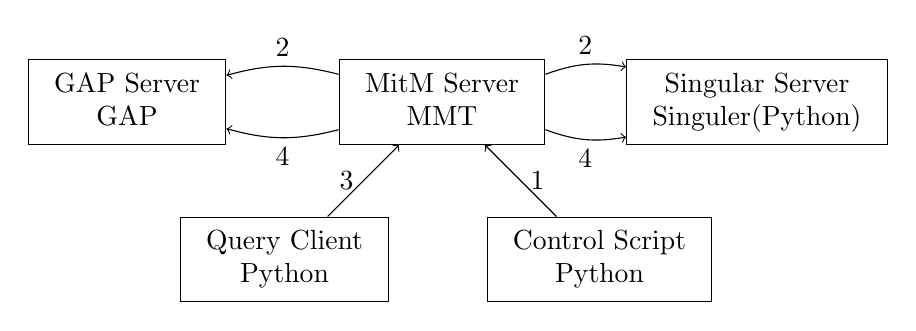
\begin{tikzpicture}[xscale=2, yscale=2]\normalsize
  \node[draw] (g) at (0,0) {
    \begin{tabular}{c}
      GAP Server \\GAP
    \end{tabular}
  };
  \node[draw] (m) at (2,0) {
    \begin{tabular}{c}
      MitM Server\\MMT
    \end{tabular}
  };
  \node[draw] (s) at (4,0) {
    \begin{tabular}{c}
      Singular Server\\Singuler(Python)
    \end{tabular}
  };
  \node[draw] (p) at (1, -1) {
    \begin{tabular}{c}
      Query Client\\Python
    \end{tabular}
  };
  \node[draw] (c) at (3, -1) {
    \begin{tabular}{c}
      Control Script\\Python
    \end{tabular}
    };
  \draw[->] (c) to node[right] {1} (m);
  \draw[->] (m) to[bend left=15] node[above] {2} (s);
  \draw[->] (m) to[bend right=15] node[above] {2} (g);
  \draw[->] (p) to node[left] {3} (m);
  \draw[->] (m) to[bend right=15] node[below] {4} (s);
  \draw[->] (m) to[bend left=15] node[below] {4} (g);
\end{tikzpicture}

%  LocalWords:  tikzpicture xscale yscale Singuler

  \caption[GAP-Singular MitM Interaction]{
    System Designed to Prove the Concept of the MitM Protocol
  }\label{fig:mitmpoc}
\end{figure}

The procedure illustrated in figure \ref{fig:mitmpoc} is as follows:
\begin{enumerate}
  \item The control script establishes an SCSCP connection with the MMT MitM 
    server and aligns the functions exposed by the CAS (GAP and Singular) with
    global symbols.
  \item The MitM server establishes SCSCP connections with the CAS server at
    provided addresses.
  \item The query client queries the MitM server for symbols from public CDs
    without any knowledge of the CAS in operation to calculate orbits of 
    polynomials.
  \item MitM server redirects the requests from the query client to the necessary
    CAS.
\end{enumerate}

\subsection{Components of the Study System}
\subsubsection{MMT MitM Server}
The MitM server is implemented as an MMT-shell extension. The integration into the
MMT ecosystem will be useful in the future for the automation of function 
alignment and type-checking of arguments. It is also queried via SCSCP as opposed 
to QMT, because currently SCSCP is more widely supported, e.g. by the GAP and 
Python packages.

\subsubsection{GAP SCSCP Server}
GAP server uses the GAP SCSCP package to expose the minimal functions needed for 
this study- the constructor for a symmetric group of size N, and a function that
takes a list and a symmetric group and returns a permutation of the list for every 
member of the symmetric group that is obtained by applying that member to every
item of the list.

\subsubsection{Singular SCSCP Server}
Since Singular currently doesn't have any support for SCSCP, the Singular SCSCP server is
written in Python using the \lstinline|scscp| and \lstinline|PySingular| python modules
and is adapted from the example code on the py-scscp repository\cite{PySCSCP}. The only
function exposed by this server is the evaluation of equality of two applications of the
DMP symbol.

\subsubsection{Controlling Client Script}
In the long term, the function alignment will be done automatically when a CAS 
informs the MitM server of its presence. Currently, however, the export of CAS 
type systems is still a work in progress, so the function alignment is done
via the MitM protocol. The job of the controlling script is thus to align the 
constructor of symmetric group of size N and the orbit of a list to their 
respective symbols in public CDs, as well as registering the ability of the 
Singular server to equate polynomials.

\subsubsection{Naive Client}
The main client that queries the MitM server has no knowledge of the underlying 
CAS. It follows the procedure:
\begin{enumerate}
  \item Create an OpenMath polynomial.
  \item Obtain a symmetric group of size that is equal to the number of variables 
    in the polynomial from MitM.
  \item Using the obtained group, query MitM for all permutations of the list 
    of variables.
  \item Create polynomials from the permutations of the list of variables.
  \item Filter out the duplicate polynomials by querying MitM for equality of 
    polynomials.
\end{enumerate}
While this is very much a brute-force algorithm to calculate an orbit of a
polynomial, it showcases the ability of the client to query the MitM server that 
is then forced to use multiple CAS without the client needing any knowledge of the
underlying systems.

\subsection{Using the System}
\subsubsection{Dependencies}
The dependencies of the software in subject of the study and instructions on
acquiring them:
\begin{itemize}
  \item \textbf{Jupyter}- installed via pip
  \item \textbf{GAP}- installed from https://github.com/gap-system/gap
  \item \textbf{Singular}- installed via package manager or from
    https://www.singular.uni-kl.de/index.php/singular-download.html
  \item \textbf{MMT}- installed from https://github.com/Uniformal/MMT
  \item \textbf{Py-SCSCP}- installed via pip
  \item \textbf{PySingular}- installed via pip or from 
    https://github.com/sebasguts/SingularPython
\end{itemize}

\subsubsection{Execution}
Instructions on running the system:
\begin{itemize}
  \item Run singular\_server.py script using python, the gap\_server.g script
    using GAP, and start MMT. From the MMT shell prompt, run 
    "file mitm\_server.msl".
  \item Run ControllingClient.py using python to set up alignments between
    MitM server and CAS servers.
  \item Start a Jupyter kernel using "jupyter notebook" and open the 
    QueryingClient.ipynb notebook. This is the example procedure that showcases
    a few examples of calculations of orbits of polynomials.
\end{itemize}

\subsection{Evaluation of the Study}
This study has implemented the MitM approach using SCSCP, showing that the MitM 
paradigm is an achievable goal. Currently, however, the MitM server acts as 
merely a proxy, redirecting SCSCP requests to CAS that know how to evaluate them.
For MitM to be a truly modular abstract algebra environment, the following
changes must be made:
\begin{itemize}
  \item A peer-to-peer connection must be made with the CAS servers, so that
    CAS servers can, in turn, query MitM if during a computation they encounter 
    a concept that lies outside their field of knowledge. In application to
    this particular case, it would be cleaner if, instead of asking MitM to 
    produce permutations of a list, the client simply queries MitM for the orbit 
    of a polynomial by defining an action of a member of the symmetric group on a 
    polynomial. GAP would then be able to calculate the orbit by making the group 
    act on the polynomial with the described action and querying MitM for 
    equality of polynomials, resulting in a linear-time algorithm instead of
    quadratic-time behaviour displayed by the current client.
  \item Alignment between CAS servers and the MitM server must be automated.
    Although manual alignment as described in this case study is usable and
    enables pinpoint alignments to be made, it is not scalable. Any CAS that aims
    to be MitM-compatible should develop a representation of its type system
    in MMT, so that, upon establishing a connection with a new CAS system, the 
    MitM server would be able to automatically align newly accessible functions 
    with symbols from public CDs. This will also enable MMT to act as more than
    a routing proxy, as it would be able to typecheck the arguments of incoming
    requests, making the MitM system more rigid.
\end{itemize}

%%% Local Variables:
%%% mode: latex
%%% TeX-master: "paper"
%%% End:

%  LocalWords:  subsubsection mitm itemize textbf centering fig:mitmpoc lstinline scscp
%  LocalWords:  Jupyter _server.msl ControllingClient.py QueryingClient.ipynb bibitem
%  LocalWords:  thebibliography
